\chapter{Related work}\label{chap:related-work}

\section*{}

This chapter presents an overview of the knowledge developed over the years in the areas of industrial robotics, environment perception, machine learning and human-robot interaction that is relevant for the development of cooperative human-robot systems capable of learning and assembling complex objects.



\section{Assembly / disassembly planning}

FF



\section{Motion planning}

Planning the coordinated motion of robotic arms \cite{Rickert2011} and grippers in assembly operations requires advanced control \cite{Stolt2015} and path planning algorithms \cite{Kuffner2000,You2012,Fontanals2014,mopl2015} and needs to take in consideration the robot hardware configuration and manipulation capabilities along with the world state and assembly knowledge \cite{Tenorth14} (such as where are the parts to be assembled and in which sequence they will be installed). This knowledge integration is critical in order to generate the assembly graph with the proper part installation sequence that ensures that the robot will be able to use its end effectors to perform all the tasks \cite{Thomas2003ATP,Thomas2011} while avoiding unintended collisions.


\subsection{Motion representation}

There are several methods for modeling the robotic motions and relative spatial disposition of objects during an automated assembly process. One of the early approaches is the \gls{tff} \cite{Mason1981,Finkemeyer2004} which provides a practical technique for defining coordinate frames along with pose, velocity and force information required to perform compliant motion using robotic manipulators. This method was later extended with the Operational Space Approach \cite{Khatib1987,DeSapio2006} in order to support dynamic and multi-body robot models. More recent methods include the Task Function Approach \cite{Samson1991} which allows to model sensors and interaction with the environment and the \gls{itasc} framework \cite{DeSchutter-ijrr2007,Smits2010} which gives the possibility to model geometric uncertainty.


\subsection{Path planning}

FF


%Articles:\\
%- A new probabilistic path planning algorithm for (dis) assembly tasks\\
%+ Development of Manipulation Planning Algorithm for a Dual-arm Robot Assembly Task\\ | You2012
%+ Integrated Grasp and Motion Planning using Independent Contact Regions\\ | Fontanals2014
%+ Knowledge-based Specification of Robot Motions\\ | Tenorth14
%- MOPL - A Multi-Modal Path Planner for Generic Manipulation Tasks
%- Assembly Planning and Task Planning - Two Prerequisites for Automated Robot Programming\\ | Thomas2011
%- Efficient assembly sequence planning using stereographical projections of c-space obstacles\\ | Thomas2003ATP



\section{Perception systems}

There is a wide range of perception algorithms and sensors that can perform object recognition \cite{Andreopoulos2013} and pose estimation, either using 2D images \cite{Marton2011,Costa2016ICARSC} or 3D data \cite{Aldoma2011,Wohlkinger2012,Lee2012,Blodow2014phd,Garcia2016}. For very specific recognition tasks, template matching techniques \cite{Lee2016} or color / shape segmentation methods (such as simple \gls{hsv} thresholding, advanced segmentation using the watershed algorithm or fitting specific shapes to the sensor data using \gls{ransac} or the Hough transform \cite{Ballard1981}) provide a simple and effective approach. For more generic perception tasks, it is usually necessary to rely on feature detection \cite{Tuytelaars2008,Filipe2014} to select reliable keypoints, feature description \cite{Gauglitz2011,Hansch2014} to characterize the geometry around each interest point and robust matching algorithms (for example \gls{ransac} coupled with \gls{knn} descriptor association and \gls{svd} pose estimation) in order to be able to recognize the objects even in cluttered environments \cite{Aldoma2016}. Other approaches rely on machine learning classifiers \cite{Rocha2015} (such as \glspl{svm}, \glspl{nn}, \glspl{dt}, \glspl{hmm}) and bag of words methods \cite{Csurka04,Nowak2006,Costa2014} in order to detect class of objects that have similar geometry and may appear in different perspectives. After the recognition stage, tracking algorithms such as Kalman \cite{Kalman1960} / particle filters \cite{Cho2006} coupled with accurate matching algorithms (for example MeanShift / CamShift \cite{Bradski1998} / \gls{icp} \cite{Besl1992}) can be used to follow the objects pose with high precision over time.

Some preliminary work has already been done in the area of 2D / 3D perception. In \cref{fig:banknote-recognition} it is shown a 2D perception system for detecting planar objects in which it is highlighted the typical processing steps required along with the most common algorithms used to estimate the 3D pose of objects from 2D images. In \cref{fig:localization-system} it is shown a similar 3D perception system that is able to perform 3D pose estimation of an object / robot from 3D sensor data.


%Articles:\\
%+ Combined 2D-3D Categorization and Classification for Multimodal Perception Systems | Marton2011
%
%Articles 2d:\\
%+ Evaluation of Interest Point Detectors and Feature Descriptors for Visual Tracking\\
%- Evaluation of interest point detectors for image information extraction\\
%- Local Invariant Feature Detectors - A Survey
%- Object Recognition from Local Scale-Invariant Features
%
%Articles 3d:\\
%+ 3DNet - Large-Scale Object Class Recognition from CAD Models\\ | Wohlkinger2012
%- 3D Visual Perception System for Bin Picking in Automotive Sub-Assembly Automation\\
%+ CAD-Model Recognition and 6DOF Pose Estimation Using 3D Cues\\ | Aldoma
%- Detecting and Segmenting Objects for Mobile Manipulation\\
%- Development of a 3D model based part recognition system for industrial applications - Main challenges\\ | Rocha2015
%+ A Global Hypothesis Verification Framework for 3D Object Recognition in Clutter
%- Scene Perception and Recognition in Industrial Environments for Human-Robot Interaction


\clearpage

\begin{figure}[H]
	\centering
	\begin{minipage}[h]{.54\textwidth}
		\centering
		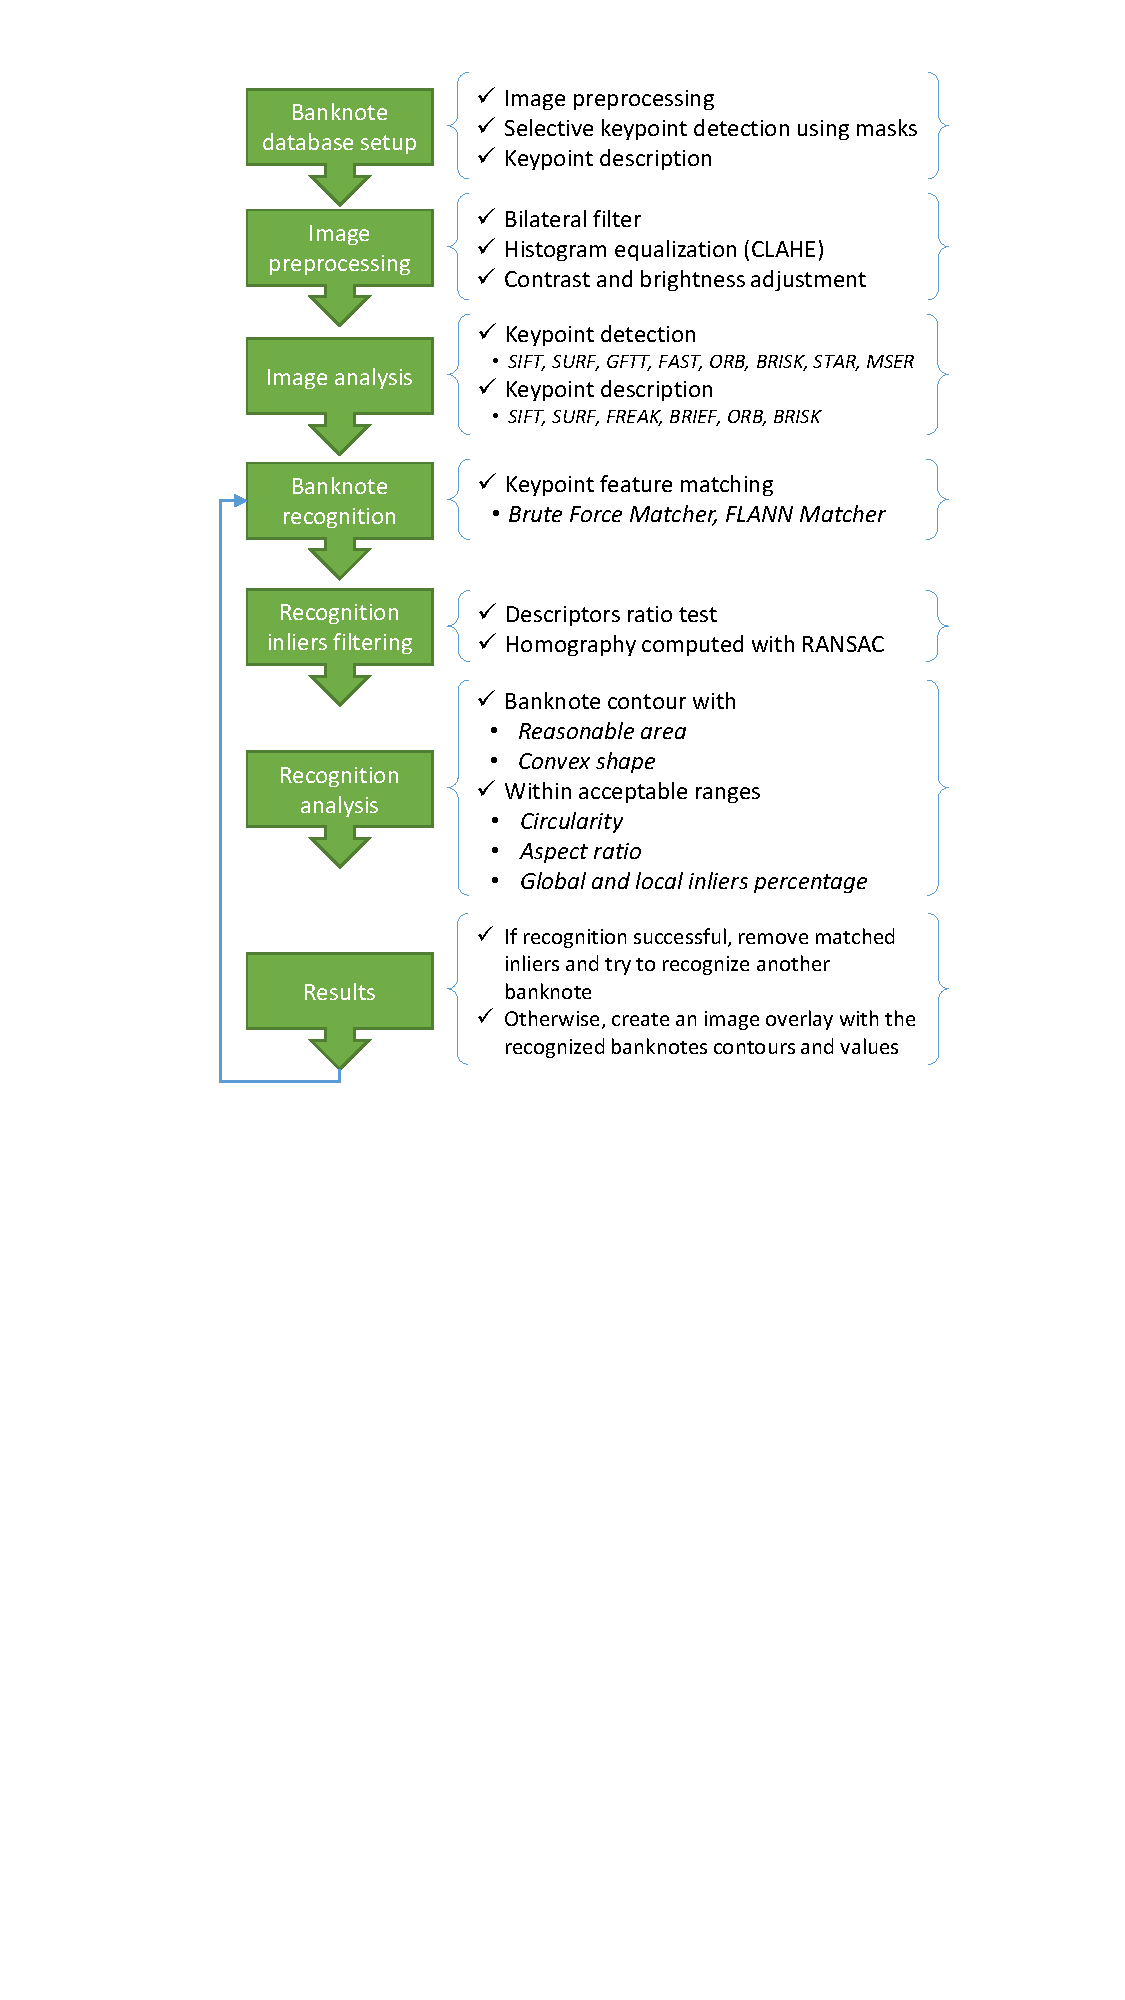
\includegraphics[width=\linewidth]{banknote-recognition/system-overview}
	\end{minipage}%
	\begin{minipage}[h]{.26\textwidth}
		\centering
		\vspace*{.37em}
		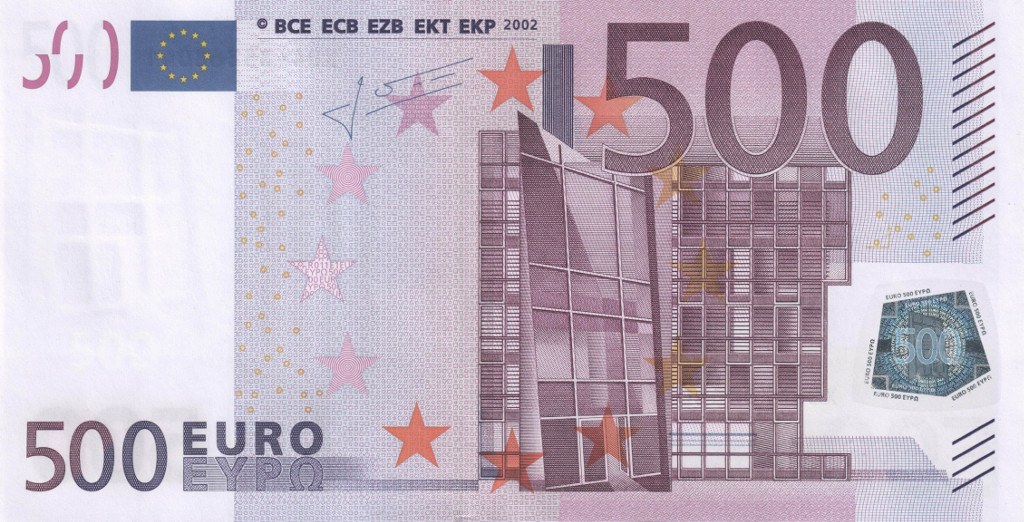
\includegraphics[width=.485\linewidth]{banknote-recognition/notes-masks/500eu-front}
		
\includegraphics[width=.485\linewidth]{banknote-recognition/notes-masks/500eu-front-mask}
		
		\vspace*{0.8em}
		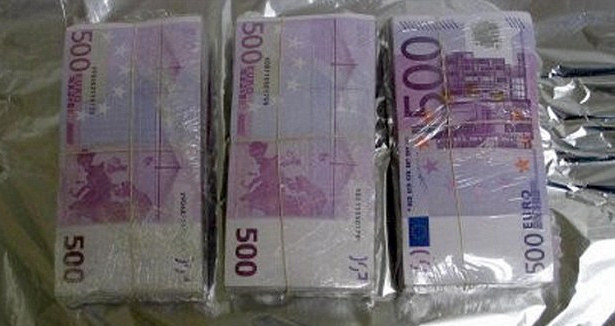
\includegraphics[width=.485\textwidth]{banknote-recognition/preprocessing/500-500-500}
		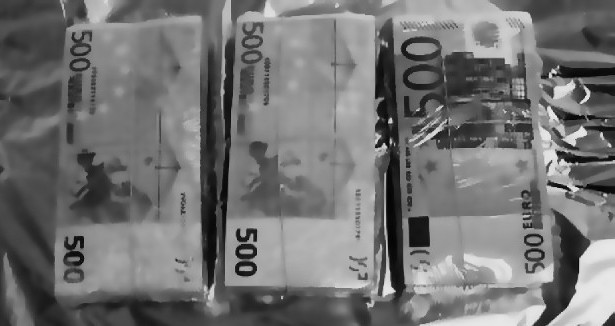
\includegraphics[width=.485\textwidth]{banknote-recognition/preprocessing/500-500-500-preprocessed}
		
		\vspace*{1.2em}
		
\includegraphics[width=.2496\textwidth]{banknote-recognition/image-resolution/500eu-front-very-low}\hfill
		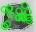
\includegraphics[width=.2496\textwidth]{banknote-recognition/image-resolution/500eu_front_currencyDB_veryLowResolution_SIFT-Detector}\hfill
		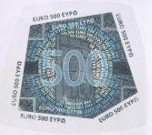
\includegraphics[width=.2499\textwidth]{banknote-recognition/image-resolution/500eu-front-medium}\hfill
		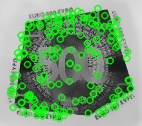
\includegraphics[width=.2499\textwidth]{banknote-recognition/image-resolution/500eu_front_currencyDB_mediumResolution_SIFT-Detector}
		
		\vspace*{.9em}
		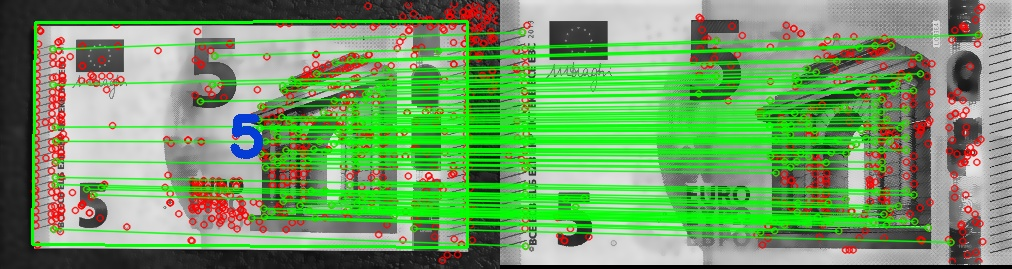
\includegraphics[width=.99\textwidth]{banknote-recognition/notes-recognition/5__(5).jpg___SIFT-Detector_SIFT-Extractor_BF-Matcher_lowQualityImageDB_globalMatch__inliersMatches__0}
		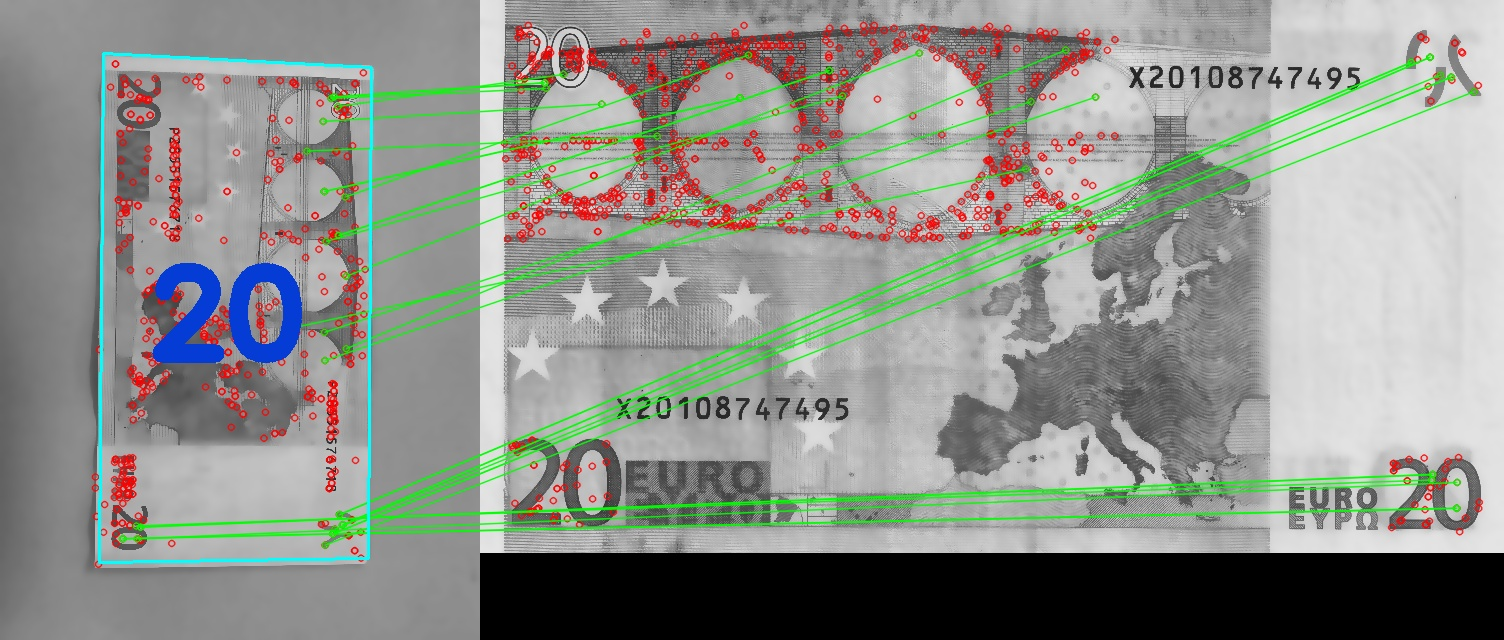
\includegraphics[width=.8\textwidth]{banknote-recognition/notes-recognition/20__(13).jpg___SIFT-Detector_SIFT-Extractor_BF-Matcher_mediumQualityImageDB_globalMatch__inliersMatches__0}
		
		\vspace*{.8em}
		
\includegraphics[width=0.75\textwidth]{banknote-recognition/notes-masks/currency-db-shapes}
		
		\vspace*{.5em}
		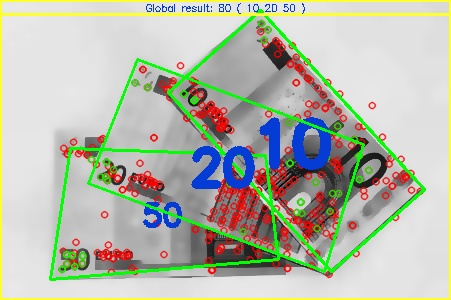
\includegraphics[width=0.8\textwidth]{banknote-recognition/notes-recognition/10-20-50.jpg___SIFT-Detector_SIFT-Extractor_BF-Matcher_dynamicQualityImageDB_globalMatch}
	\end{minipage}
	\caption[Overview of a 2D perception system for planar object recognition]{Overview of a 2D perception system for planar object recognition \cite{Costa2016ICARSC}}
	\label{fig:banknote-recognition}
\end{figure}

\begin{figure}[H]
	\centering
	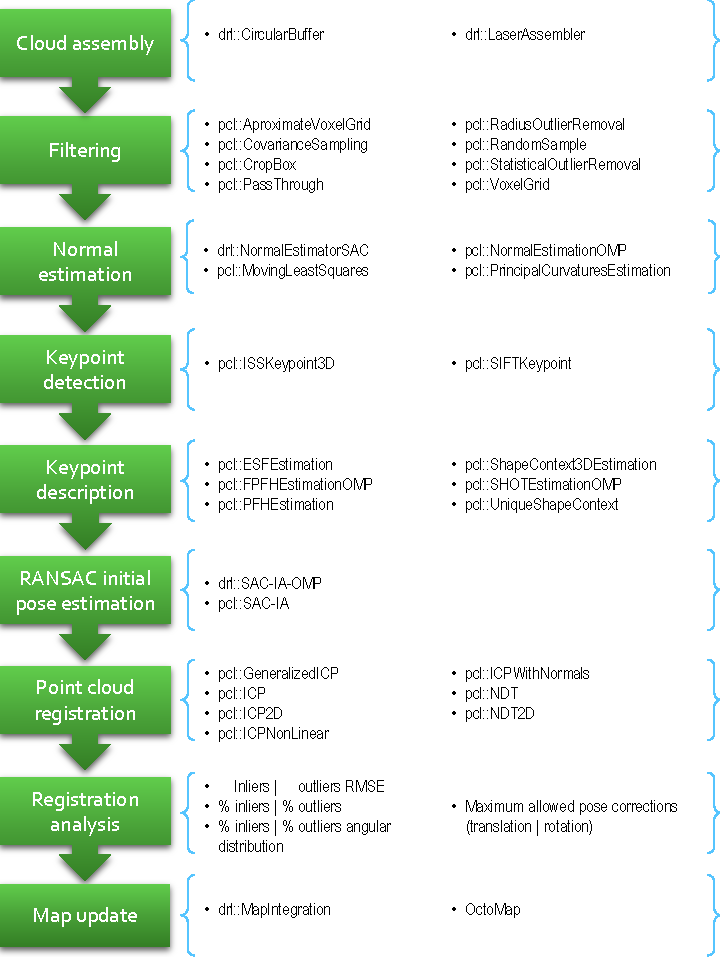
\includegraphics[height=.41\textheight]{self-localization/localization-system-modules}
	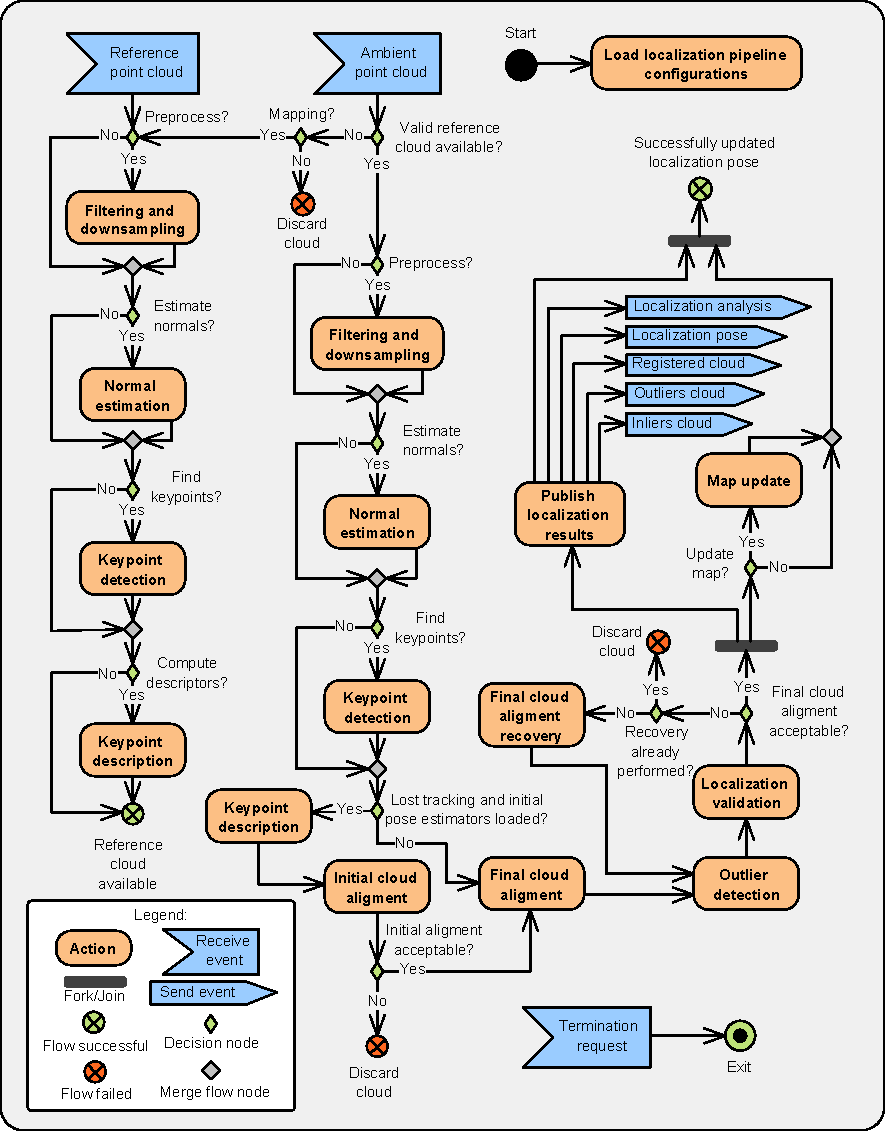
\includegraphics[height=.41\textheight]{self-localization/localization-system-overview}
	\caption[Overview of a 3D perception system for object / robot pose estimation]{Overview of a 3D perception system for object / robot pose estimation \cite{Costa2016Elsevier}}
	\label{fig:localization-system}
\end{figure}



\section{Knowledge management}

Creation and management of reusable knowledge across robots with different hardware configurations is a challenging task that can be solved by using cloud robotics coupled with ontology databases and skill frameworks. The next sections present a brief overview of the application of these approaches to robotic assembly systems.


\subsection{Ontologies}

Ontologies allow to model world information in a structured and object oriented approach \cite{Lemaignan2012,Stenmark2015}, which can be useful to store information about the environment, robot capabilities, configurations, sensors, tools as well as detailed descriptions of the assembly objects \cite{Perzylo2015}, such as its \gls{cad} data, their spatial disposition during the assembly process and other meta-information (for example the force / torque or direction required to insure proper coupling of objects).

%Articles:\\
%+ An ontology for CAD data and geometric constraints as a link between product models and semantic robot task descriptions | Perzylo2015
%+ Knowledge-based instruction of manipulation tasks for industrial robotics | Stenmark2015


\subsection{Skills}

Automation of assembly operations in industrial applications \cite{Thomas2001,Patel2012} is a multidisciplinary challenging task that orchestrates and manages the assembly operation graph using \glspl{fsm} \cite{Smits2010,Stefan2014} and requires the integration of the robot motion planners with the gripping tools \cite{Thomas2015} along with the perception systems. Moreover, these assembly operations need to be reusable \cite{Andersen2014,Butting2016} between robots with different hardware configurations \cite{Thomas2002} but with equivalent assembly capabilities. This can be achieved by modeling assembly operations as abstract skills \cite{aimm2012,Pedersen2014,Holz2015} that can be executed with fault tolerance \cite{ThomasICRA2003} on top of a primitive software layer that models reusable operations, which in turn are executed on top of a device layer that transforms the abstract knowledge into robot perception and motion commands (diagram of skill based assembly system shown in \cref{fig:skiros}). These skills can either be taught by a human operator by demonstration or be automatically extracted from \gls{cad} / \gls{sop} analysis \cite{Lavoue2005,Tenorth2013cad} or also retrieved from a high level description such as \gls{uml}/P statecharts \cite{ThomasICRA2013}.


\begin{figure}[H]
	\centering
	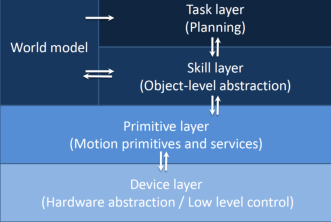
\includegraphics[width=0.5\linewidth]{related-work/skiros}
	\caption[Skill-based Architecture SkiROS]{Skill-based Architecture SkiROS \cite{Holz2015}}
	\label{fig:skiros}
\end{figure}


%Articles:\\
%+ A new skill based robot programming language using uml-p statecharts\\
%+ A system for automatic planning, evaluation and execution of assembly sequences for industrial robots\\
%- A unified notation for serial, parallel, and hybrid kinematic structures
%+ Enabling robots in small-part assembly lines\\
%+ Flexible assembly through integrated assembly sequence planning and grasp planning\\
%+ Modeling Reusable, Platform-Independent Robot Assembly Processes
%- A new framework for task oriented sensor based robot programming and verification\\
%+ A Skill-Based System for Object Perception and Manipulation for Automating Kitting Tasks\\
%+ Definition of Hardware-Independent Robot Skills for Industrial Robotic Co-workers\\
%+ Error-tolerant execution of complex robot tasks based on skill primitives\\
%- Skills for Vision-based Applications in Robotics Application to aeronautics assembly pilot station



\subsection{Cloud robotics}

Given the reusable nature of assembly operations, cloud robotics can provide a communication and storage architecture for the distribution of new learned skills across a fleet of robots \cite{Tenorth2013,Stenmark2015T} and could also allow to offload heavy processing operations, such as data mining \cite{Witten2005} and cognition related tasks \cite{Beetz2010,Tenorth2013k,Saxena2014,Beetz2015} from the robots embedded systems into more powerful processing servers \cite{Hunziker2013}.

%Articles:\\
%- On Distributed Knowledge Bases for Robotized Small-Batch Assembly\\
%+ KnowRob - A Knowledge Processing Infrastructure for cognition-enabled robots\\ | Tenorth2013
%+ OPEN-EASE - A Knowledge Processing Service for Robots and Robotics - AI Researchers\\ | Beetz2015
%+ Representation and exchange of knowledge about actions, objects, and environments in the roboearth framework\\ | Tenorth2013
%+ RoboBrain - Large-Scale Knwoledge Engine for Robots\\ | Saxena2014
%+ CRAM - A Cognitive Robot Abstract Machine for Everyday Manipulation in Human Environments\\ | Beetz2010
%+ Rapyuta - The RoboEarth Cloud Engine | Hunziker2013
%+ Data Mining - Practical Machine Learning Tools and Techniques (3rd Ed) | Witten2005



\section{Teaching systems}

There are several approaches for teaching new skills to robots, ranging from advanced teach pendent / lead through programming, to the easy and intuitive usage of task level and \gls{cad} based specifications using \gls{ar} or tactile interfaces \cite{Perzylo2015a}. However, the teaching can be faster and more intuitive if the robot manages to learn new assembly knowledge \cite{tensorflow} by human demonstration \cite{Argall2009,Hamabe2015,Wang2015} in which the systems tracks the human operator movements and objects in order to build the assembly graph and the underlying \gls{fsm} that contains the order and coupling operations required. Moreover, in the case of anthropomorphic robots it can use the human arm movements as a starting point for the robot path planning \cite{Zanchettin2012} that is required to perform the assembly operations without unintended collisions.

%\begin{figure}[H]
%	\centering
%	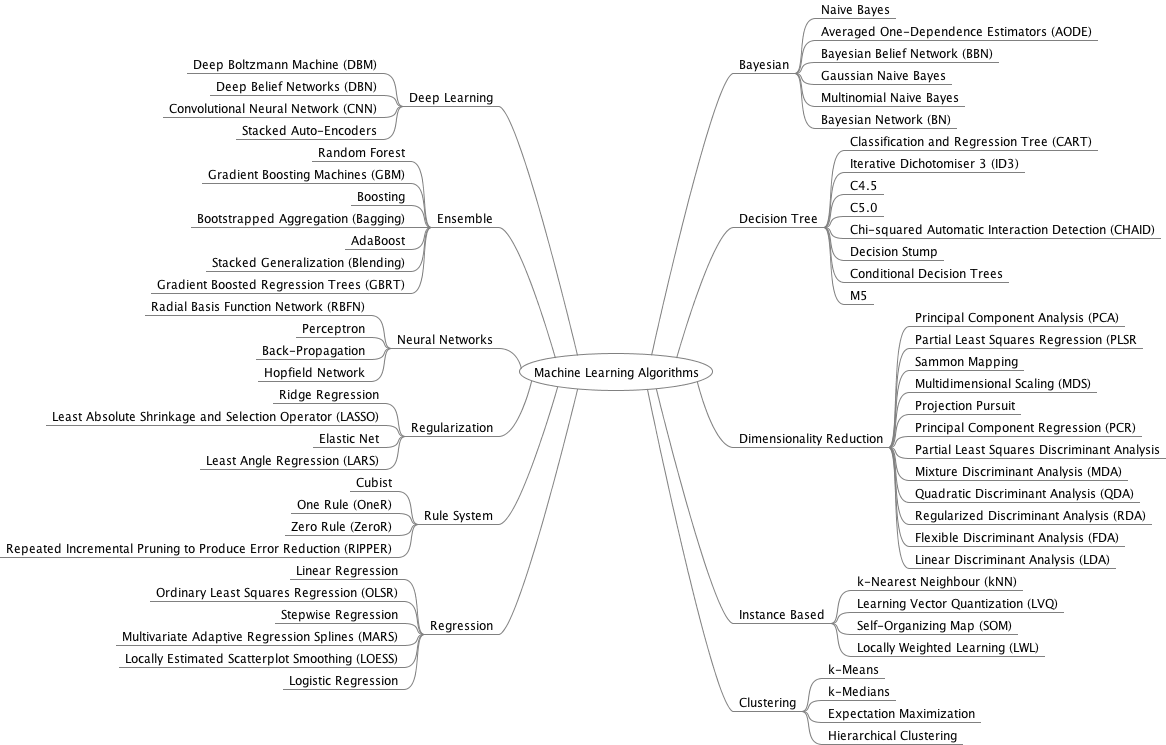
\includegraphics[width=\linewidth]{related-work/machinelearningalgorithms}
%	\caption[Machine learning algorithms mind map]{Machine learning algorithms mind map\protect\footnotemark}
%	\label{fig:machinelearningalgorithms}
%\end{figure}
%\footnotetext{\url{https://jixta.wordpress.com/2015/07/17/machine-learning-algorithms-mindmap}}

%Articles:\\
%- Efficient Model Learning from Joint-Action Demonstrations for Human-Robot Collaborative Tasks
%- Robust control of force-coupled human–robot-interaction in assembly processes\\
%+ Toward Efficient Robot Teach-In and Semantic Process Descriptions for Small Lot Sizes | Perzylo2015a
%+ TensorFlow - Large-Scale Machine Learning on Heterogeneous Distributed Systems | tensorflow
%+ A Programming by Demonstration System for Human-Robot Collaborative Assembly Tasks
%+ Multi-class Assembly Parts Recognition using Composite Feature and Random Forest for Robot Programming by Demonstration



\section{Human Machine Interaction systems}

There is a wide range of technologies that allow the exchange of information between humans and machines \cite{Goodrich2008}, from the typical display devices (screens, projectors) to natural interaction using visual and audio \cite{Yan2014} communication protocols. The next sections provide a brief overview of the human machine interaction systems that are useful for cooperative assembly operations.

%Articles:\\
%- A Survey on Perception Methods for Human-Robot Interaction in Social Robots\\ | Yan2014
%- Human-Robot Interaction - A Survey | Goodrich2008


\subsection{Augmented reality}

\gls{ar} interfaces \cite{Bimber2005} offer an immersive way of exchanging information between a human operator and a robot / machine \cite{Kollatsch2014,Gaschler2014,Dini2015,Michalos2016}. This can be achieved with a wide range of devices, such as projectors, smart glasses, tablets, smart-phones, \gls{vr} headsets, among others. Projectors allow to perform accurate environment marking of information \cite{Tan2013,Fujimoto2014}, which is useful for assisting the operator in new complex tasks (such as assembly or maintenance) and also allow the operator to perform cutting / welding operations faster by avoiding manual measurements (example in \cref{fig:laser-projection}). Smart glasses (such as the Microsoft HoloLens\footnote{\url{https://www.microsoft.com/microsoft-hololens/en-us}} shown in \cref{fig:hololens}) offer a more flexible alternative which is more suitable for providing guiding information while the operator is performing complex and long jobs. Screens with rear mounted sensors (such as 2D / stereo cameras, RGB-D, \gls{tof}) provide a quick and low cost approach for adding environment annotations which are useful for quick assembly / maintenance operations (example in \cref{fig:ar-assembly}). Finally, \gls{vr} headsets (such as the HTC Vive shown in \cref{fig:htc-vive}) provide an immersive environment for teaching the robot / operator without requiring access to all the physical objects / robots / environment layout.

\begin{figure}[H]
	\begin{floatrow}[2]
		\ffigbox[\FBwidth]
		{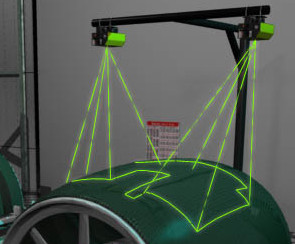
\includegraphics[height=.21\textheight]{related-work/laser-projection}}
		{\caption[Projection mapping of cutting information]{Projection mapping of cutting information\protect\footnotemark}\label{fig:laser-projection}}
		\ffigbox[\FBwidth]
		{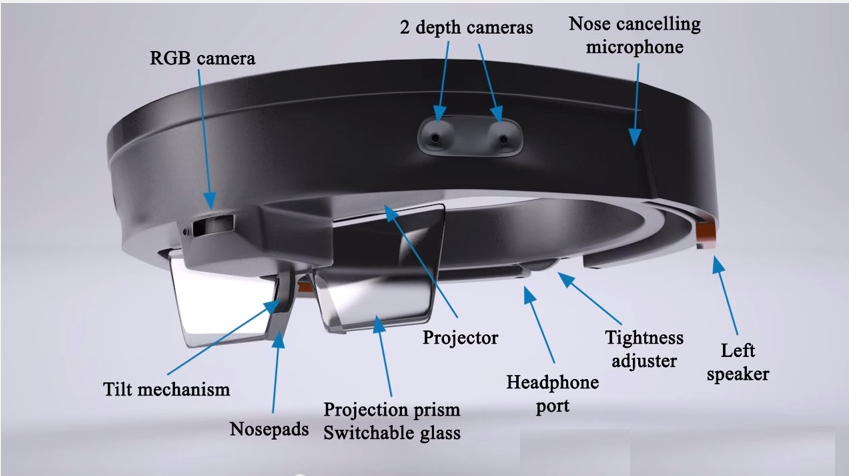
\includegraphics[height=.21\textheight]{related-work/hololens}}
		{\caption[Microsoft HoloLens]{Microsoft HoloLens\protect\footnotemark}\label{fig:hololens}}
	\end{floatrow}
\end{figure}
\footnotetext[\the\numexpr\value{footnote}-1\relax]{\url{http://www.3dgage.com/laserprojection.html}}
\footnotetext[\value{footnote}]{\url{http://www.nasdaq.com/article/himax-technologiess-a-top-augmented-realityvirtual-reality-play-cm453889}}

\begin{figure}[H]
	\begin{floatrow}[2]
		\ffigbox[\FBwidth]
		{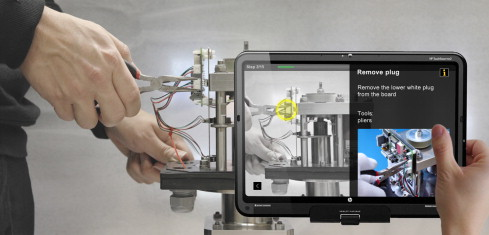
\includegraphics[height=.162\textheight]{related-work/ar-assembly}}
		{\caption[Training of a assembly task]{Training of an assembly task \cite{Webel2013}}\label{fig:ar-assembly}}
		\ffigbox[\FBwidth]
		{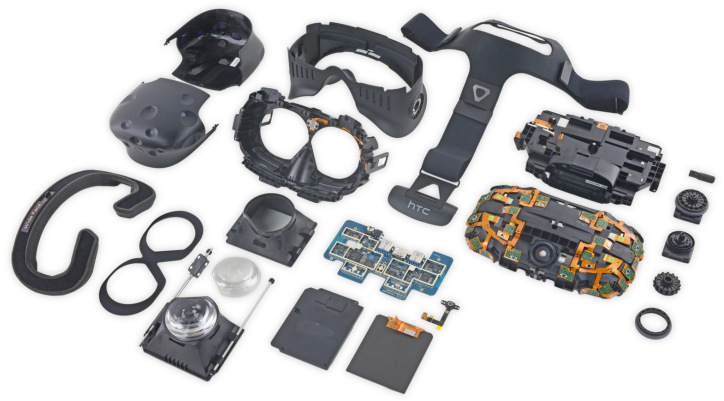
\includegraphics[height=.162\textheight]{related-work/htc-vive}}
		{\caption[HTC Vive virtual reality headset]{HTC Vive virtual reality headset\protect\footnotemark}\label{fig:htc-vive}}
	\end{floatrow}
\end{figure}
\footnotetext{\url{https://techcrunch.com/2016/04/26/teardown-of-htc-vive-highlights-the-headsets-differences-from-oculus-rift}}


%Articles:\\
%- Intuitive Robot Tasks with Augmented Reality and Virtual Obstacles\\
%+ iSarProjection - A KinectFusion Based Handheld Dynamic Spatial Augmented Reality System\\ | Tan2013
%+ Spatial Augmented Reality Merging Real and VirtualWorlds\\ | Bimber2005
%+ The Office of the Future - A Unified Approach to Image-Based Modeling and Spatially Immersive Displays | Raskar1998
%+ CAD model based virtual assembly simulation, planning and training
%
%Articles projection mapping:\\
%- A Flexible Fringe Projection Vision System with Extended Mathematical Model for Accurate Three-Dimensional Measurement\\
%- Geometrically-Correct Projection-Based Texture Mapping onto a Deformable Object



\subsection{Human-robot cooperation}

Gesture recognition of operators hand movements \cite{Oikonomidis2012,Gleeson2013} is an important task when learning new assembly skills from demonstration \cite{Nikolaidis2013} or when capturing new operator commands. Moreover, effective cooperation \cite{Adorno2011} and exchange of information between humans and robots \cite{Pandey2012,Putz2014} requires perception of the human body movements \cite{Roitberg2014} in order to learn kinematic configurations for assembly, keep tracking the objects even if they are temporarily occluded and also recognize the operator intentions to detect when the robot should initiate or stop the interaction.


%Articles:\\
%- Analysis of Task-Based Gestures in Human-Robot Interaction\\
%+ Gestures for Industry - Intuitive Human-Robot Communication from Human Observation\\
%+ Human Activity Recognition in the Context of Industrial Human-Robot Interaction\\ | Roitberg2014
%- Human-Robot Communication for Collaborative Assembly
%
%Articles:\\
%- Coordination Mechanisms in Human-Robot Collaboration\\
%- Development of Collaborative Robots for Flexible Human Integrated Assembly Automation\\
%- Dynamic Emotion-Based Human-Robot Collaborative Assembly in Manufacturing\\
%- Human-Robot Collaborative Assembly by On-line Human Action Recognition Based on an FSM Task Model\\
%- Human-Robot Interaction for Cooperative Manipulation - Handing Objects to One Another\\
%- Identifying Nonverbal Cues for Automated Human-Robot Turn-taking\\
%- Information Support Development with Human-Centered Approach for Human-Robot Collaboration in Cellular Manufacturing



\section{Natural language processing}

Natural language processing \cite{Manning1999,Jurafsky2000,Manning2008} of voice commands or unstructured textual representations (using frameworks such as GATE\footnote{\url{https://gate.ac.uk}}, CoreNLP\footnote{\url{http://stanfordnlp.github.io/CoreNLP/}}, NLTK\footnote{\url{http://www.nltk.org}}) can be very useful for extracting assembly information from \glspl{sop} / operator manuals and speedup the robot learning process \cite{Tenorth2010,Stenmark2013,Stenmark2014,Stenmark2016} (for example identifying which objects will be assembled using \gls{ner} \cite{Ekbal2012,Rami2014} and also in which order and their approximate spatial distribution).

%Articles:\\
%- Connecting natural language to task demonstrations and low-level control of industrial robots\\
%- Describing constraint-based assembly tasks in unstructured natural language\\
%- Natural Language Programming of Industrial Robots\\
%- Understanding and Executing Instructions for Everyday Manipulation Tasks from the World Wide Web | Tenorth2010




\section{Related research groups}

Automation of assembly operations is a multidisciplinary research field with a very active community in both the academia and industry. The list below presents some of the most important research groups and projects in the areas of cognitive systems and industrial robotics assembly.

\begin{table}[H]
	\caption{Related research groups and projects}
	\tabulinesep = 0.7ex
	\centering
	\scriptsize
	\begin{tabu} { X[m,c] X[0.9,m,c] X[1.2,m,c] X[1.8,m,c] }
		\rowfont{\bfseries\itshape} Research institute & Research group & Related projects & Related research areas \\
		\hline
		\href{http://www.en.aau.dk}{Aalborg University} &
		\href{http://robotics-automation.aau.dk}{Robotics and Automation} &
		\href{http://www.acat-project.eu/}{ACat} | \href{http://carlosproject.eu/}{CARLoS} | \href{http://tapas-project.eu/}{TAPAS} &
		Cognitive and manufacturing robotics Human-Machine Interaction \\

%		\tabucline[1pt on 1.5pt off 3pt]{-}
%		\href{https://www.b-tu.de/en}{Brandenburg University of Technology} &
%		\href{https://www.b-tu.de/en/research/research-projects/innovation-center-modern-industry-brandenburg}{Innovation Centre for Modern Industry} &
%		\href{http://www.smerobotics.org/AUTOMATICA/exhibit-06-2016.html}{SMERobotics} &
%		Industrial robotics | Robotic assembly \\

		\tabucline[1pt on 1.5pt off 3pt]{-}
		\href{http://www.cmu.edu}{Carnegie Mellon University} &
		\href{https://www.ri.cmu.edu}{CMU Robotics Institute} &
		\href{http://www.frc.ri.cmu.edu/projects/ace}{ACE} | \href{https://www.ri.cmu.edu/research_project_detail.html?project_id=550\&menu_id=261}{ANS} | \href{http://www.nrec.ri.cmu.edu/projects/arms}{ARM-S} | \href{https://www.ri.cmu.edu/research_project_detail.html?project_id=579\&menu_id=261}{Cell Tracking} &
		Bioengineering | Computer vision | Mobile robotics \\

		\tabucline[1pt on 1.5pt off 3pt]{-}
		\href{https://www.tu-chemnitz.de}{Chemnitz University of Technology} &
		\href{https://www.tu-chemnitz.de/etit/robosys/index.php.en}{Robotics and Human-Machine Interaction} &
		\href{http://www.euroc-project.eu/index.php?id=challenger_cutrob}{CUTRob+} | \href{http://www.drematrix.de/projects/hroc-human-robot-cooperation/}{H-RoC} \href{http://www.smerobotics.org/AUTOMATICA/exhibit-02-2016.html}{SMERobotics} &
		2D / 3D perception | Human-Robot Interaction | Robotic assembly \\

%		\tabucline[1pt on 1.5pt off 3pt]{-}
%		\href{http://www.dti.dk}{Danish Technological Institute} &
%		\href{http://www.dti.dk/services/robot-technology/products/23617}{Industrial Production} &
%		\href{http://www.dti.dk/projects/project-intelligent-robots-for-handling-of-flexible-objects/35515}{IRFO} | \href{http://www.smerobotics.org/AUTOMATICA/exhibit-04-2016.html}{SMERobotics} &
%		Bioengineering | Computer vision Industrial and service robotics \\

		\tabucline[1pt on 1.5pt off 3pt]{-}
		\href{https://www.tue.nl/en}{Eindhoven University of Technology} &
		\href{https://www.tue.nl/en/research/research-institutes/robotics-research/research-groups/control-systems-technology/}{Control Systems Technology} &
		\href{https://www.tue.nl/en/research/research-institutes/robotics-research/projects/r3-cop/}{R3-Cop} | \href{http://roboearth.org/}{RoboEarth} | \href{https://www.tue.nl/en/research/research-institutes/robotics-research/projects/rose/}{ROSE} &
		Bioengineering | Service and health-care robotics \\

		\tabucline[1pt on 1.5pt off 3pt]{-}
		\href{http://www.fortiss.org/en/home/}{fortiss} &
		\href{http://www.fortiss.org/en/research/research-topic/robotics/}{Robotics} &
		\href{http://www.fortiss.org/en/research/projects/fortiss_future_factory_f/}{f++} | \href{https://www.humanbrainproject.eu/}{Human Brain Project} \href{http://www.james-project.eu/}{JAMES} | \href{http://www.smerobotics.org/AUTOMATICA/exhibit-03-2016.html}{SMERobotics} &
		Human-Machine Interaction | Industrial and cognitive robotics \\

		\tabucline[1pt on 1.5pt off 3pt]{-}
		\href{https://www.fraunhofer.de/en.html}{Fraunhofer Institute} &
		\href{http://www.ipa.fraunhofer.de/en.html}{Manufacturing Engineering and Automation} &
		\href{http://www.project-leanautomation.eu}{LIAA} | \href{http://www.pisa-ip.org}{PiSA} | \href{http://www.fp7rosetta.org}{ROSETTA} \href{http://www.smerobot.org}{SMERobot} | \href{http://www.smerobotics.org/AUTOMATICA/exhibit-08-2016.html}{SMERobotics} \href{http://www.symbio-tic.eu}{SYMBIO-TIC} &
		Bioengineering | Biomechatronics Human-Machine Interaction | Industrial and service robotics \\

		\tabucline[1pt on 1.5pt off 3pt]{-}
		\href{http://www.dlr.de/dlr/en}{German Aerospace Center} &
		\href{http://www.dlr.de/rm/en}{Robotics and Mechatronics Center} &
		\href{http://www.arcas-project.eu}{ARCAS} | \href{http://www.phriends.eu/}{PHRiENDS} \href{http://www.saphari.eu}{SAPHARI} | \href{http://tapas-project.eu/}{TAPAS} &
		Human-Machine Interfaces | Mechatronics Robotics perception and cognition \\

		\tabucline[1pt on 1.5pt off 3pt]{-}
		\href{http://www.tekniker.es/en}{IK4-Tekniker} &
		\href{http://www.tekniker.es/en/automation-and-industrial-robotics}{Smart and Autonomous System} &
		\href{http://fourbythree.eu/}{FourByThree} | \href{http://www.robo-partner.eu}{Robo-Partner} \href{http://www.xact-project.eu}{X-act} &
		Human-Machine Interaction | Industrial and service robotics | Robotic assembly \\

		\tabucline[1pt on 1.5pt off 3pt]{-}
		\href{http://www.lunduniversity.lu.se/}{Lund University} &
		\href{http://www.control.lth.se/Research/Robotics.html}{Robotics Lab} &
		\href{http://www.control.lth.se/Research/Robotics/prace-project.html}{PRACE} | \href{http://www.fp7rosetta.org}{ROSETTA} \href{http://h2020sarafun.eu}{SARAFun} | \href{http://rss.cs.lth.se/projects/completed/siaras/}{SIARAS} \href{http://www.smerobot.org}{SMERobot} | \href{http://www.smerobotics.org/AUTOMATICA/exhibit-09-2016.html}{SMERobotics} &
		Computer vision | Industrial robotics | Task and skills learning by demonstration \\

		\tabucline[1pt on 1.5pt off 3pt]{-}
		\href{http://web.mit.edu/}{Massachusetts Institute of Technology} &
		\href{https://interactive.mit.edu/about/vision}{Interactive Robotics Group} &
		\href{https://interactive.mit.edu/research}{Shared Mental Models for Human-Robot Teaming} &
		Human-Robot Interaction | Machine Learning | Mobile robotics \\

		\tabucline[1pt on 1.5pt off 3pt]{-}
		\href{http://www.osrfoundation.org}{Open Source Robotics Foundation} &
		\href{http://www.osrfoundation.org/osrf-projects/}{Robotics} &
		\href{http://gazebosim.org/}{Gazebo} | \href{http://www.ros.org/}{ROS} | \href{http://rosindustrial.org/}{ROS Industrial} &
		Industrial and service robotics \\

		\tabucline[1pt on 1.5pt off 3pt]{-}
		\href{http://www.tu-darmstadt.de}{Technical University of Darmstadt} &
		\href{http://www.ausy.tu-darmstadt.de}{Autonomous Systems} &
		\href{http://3rdhandrobot.eu}{3rdHand} | \href{http://bimrob.ausy.tu-darmstadt.de/Main/HomePage}{BIMROB} | \href{http://www.gert-project.eu/project/project-summary}{GeRT} \href{http://tacman.eu}{TACMAN} &
		Cognitive systems | Human-Robot Interaction | Machine Learning \\

		\tabucline[1pt on 1.5pt off 3pt]{-}
		\href{http://www.tum.de/en}{Technical University of Munich} &
		\href{http://www6.in.tum.de/Main/Research}{Robotics and Embedded Systems} &
		\href{https://www.humanbrainproject.eu/}{HBP} | \href{http://www6.in.tum.de/Main/ResearchJahir}{JAHIR} | \href{http://www6.in.tum.de/Main/ResearchJast}{JAST} \href{http://roboearth.org/}{RoboEarth} | \href{https://robohow.eu}{RoboHow} \href{http://www.saphari.eu}{SAPHARI} | \href{http://www.shrine-project.eu}{SHRINE} &
		Cognitive systems | Computer vision Human-Robot Interaction | Industrial and health-care robotics \\

		\tabucline[1pt on 1.5pt off 3pt]{-}
		\href{http://www.birmingham.ac.uk}{University of Birmingham} &
		\href{https://www.cs.bham.ac.uk/research/groupings/robotics/}{Intelligent Robotics Lab} &
		\href{https://cogimon.eu}{CogIMon} | \href{https://www.cs.bham.ac.uk/research/groupings/robotics/projects/cogx}{CogX} | \href{https://www.cs.bham.ac.uk/~rwd/research/gert-main.php}{GeRT} \href{http://www.pacman-project.eu/}{PaCMan} | \href{http://strands.acin.tuwien.ac.at/}{STRANDS} &
		Cognitive systems | Object manipulation and assembly | Service robotics \\

		\tabucline[1pt on 1.5pt off 3pt]{-}
		\href{http://www.uni-bremen.de/en.html}{University of Bremen} &
		\href{http://ai.uni-bremen.de/research/ias}{Intelligent Autonomous Systems} &
		\href{http://www.actioncores.org/}{PRAC} | \href{http://www.open-ease.org/}{openEASE} \href{http://roboearth.org/}{RoboEarth} | \href{https://robohow.eu}{RoboHow} \href{http://www.robosherlock.org/}{RoboSherlock} | \href{http://www.saphari.eu}{SAPHARI} &
		2D / 3D perception | Cognitive systems Machine Learning | Natural Language Processing | Service robotics \\

		\tabucline[1pt on 1.5pt off 3pt]{-}
		\href{http://www.bristol.ac.uk}{University of Bristol} &
		\href{http://www.brl.ac.uk/}{Bristol Robotics Laboratory} &
		\href{http://www.brl.ac.uk/research/researchthemes/nonlinearcontrolinrobotics/anthropomorphicdynamics.aspx}{ANDy} | \href{http://www.chrisfp7.eu/}{CHRIS} \href{http://echord.eu/}{ECHORD++} | \href{http://introbotics.eu/}{INTRO} \href{http://www.brl.ac.uk/research/researchthemes/robotvision/moetmanipulationofobjects.aspx}{MOET} | \href{http://www.robosafe.org/}{RoboSafe} &
		Computer vision | Bioengineering Human-Robot Interaction | Health-care robotics | Mechatronics \\

		\tabucline[1pt on 1.5pt off 3pt]{-}
		\href{http://www.sdu.dk/en}{University of Southern Denmark} &
		\href{http://www.sdu.dk/en/om_sdu/institutter_centre/sdurobotics}{SDU Robotics} &
		\href{http://caro.sdu.dk/index.php/projects/projectslist?view=project\&task=show\&id=6}{CARMEN} | \href{http://www.reconcell.eu/}{ReconCell} \href{http://www.xperience.org/}{Xperience} &
		Cognitive systems | Industrial and service robotics | Robotic assembly \\

		\tabucline[1pt on 1.5pt off 3pt]{-}
		\href{http://en.univ-toulouse.fr}{University of Toulouse} &
		\href{https://www.laas.fr/public/en/laboratory-presentation}{LAAS} &
		\href{http://www.chrisfp7.eu/}{CHRIS} | \href{http://www.dexmart.eu}{Dexmart} | \href{http://www.agence-nationale-recherche.fr/?Project=ANR-10-CORD-0025}{ICARO} \href{http://www.saphari.eu/}{SAPHARI} &
		Cognitive systems | Human-Machine Interaction | Object manipulation \\
	\end{tabu}
	\label{tab:label}
\end{table}



%\section{Related research projects}
%
%Automation of assembly operations is a multidisciplinary research field with a very active community in both academia and also in the industry. In the list below is presented some of the most important projects in the area of cognitive robotics in the last decades.
%
%
%\begin{itemize}
%	\item \glsentrytext{acat}\footnote{\url{http://www.acat-project.eu}} - \glsdesc{acat}
%	\item \glsentrytext{arms}\footnote{\url{http://www.nrec.ri.cmu.edu/projects/arms}} - \glsdesc{arms}
%	\item \glsentrytext{charm}\footnote{\url{http://charm.sites.olt.ubc.ca}} - \glsdesc{charm}
%	\item \glsentrytext{chris}\footnote{\url{http://www.chrisfp7.eu}} - \glsdesc{chris}
%	\item \glsentrytext{cogimon}\footnote{\url{https://cogimon.eu}} - \glsdesc{cogimon}
%	\item FourByThree\footnote{\url{http://fourbythree.eu}}
%	\item \glsentrytext{jahir}\footnote{\url{http://www6.in.tum.de/Main/ResearchJahir}} - \glsdesc{jahir}
%	\item \glsentrytext{james}\footnote{\url{http://www.james-project.eu}} - \glsdesc{james}
%	\item \glsentrytext{jast}\footnote{\url{http://www6.in.tum.de/Main/ResearchJast}} - \glsdesc{jast}
%	\item \glsentrytext{liaa}\footnote{\url{http://www.project-leanautomation.eu}} - \glsdesc{liaa}
%	\item \glsentrytext{pisa}\footnote{\url{http://www.pisa-ip.org}} - \glsdesc{pisa}
%	\item \glsentrytext{reconcell}\footnote{\url{http://www.reconcell.eu}} - \glsdesc{reconcell}
%	\item RoboEarth\footnote{\url{http://roboearth.org}}
%	\item RoboHow\footnote{\url{https://robohow.eu}}
%	\item Robo-Partner\footnote{\url{http://www.robo-partner.eu}}
%	\item \glsentrytext{rosetta}\footnote{\url{http://www.fp7rosetta.org}} - \glsdesc{rosetta}
%	\item ROS-Industrial\footnote{\url{http://rosindustrial.org}}
%	\item \glsentrytext{saphari}\footnote{\url{http://www.saphari.eu}} - \glsdesc{saphari}
%	\item \glsentrytext{sarafun}\footnote{\url{http://h2020sarafun.eu}} - \glsdesc{sarafun}
%	\item \glsentrytext{shrine}\footnote{\url{http://www.shrine-project.eu}} - \glsdesc{shrine}
%	\item \glsentrytext{symbiotic}\footnote{\url{http://www.symbio-tic.eu}} - \glsdesc{symbiotic}
%	\item SME-Robot\footnote{\url{http://www.smerobot.org}}
%	\item SME-Robotics\footnote{\url{http://www.smerobotics.org}}
%	\item \glsentrytext{xact}\footnote{\url{http://www.xact-project.eu}} - \glsdesc{xact}
%	\item \glsentrytext{tapas}\footnote{\url{http://www.tapas-project.eu}} - \glsdesc{tapas}
%\end{itemize}



\section{Related journals}

A list with the most prestigious journals in robotics is presented below.

\begin{itemize}[leftmargin=2em]
	\item \href{http://ijr.sagepub.com/}{IJR} - SAGE International Journal of Robotics Research (\href{http://www.scimagojr.com/journalsearch.php?q=18050\&tip=sid\&clean=0}{SJR} - 4.184)
	\item \href{http://ieeexplore.ieee.org/xpl/RecentIssue.jsp?punumber=9424}{TII} - IEEE Transactions on Industrial Informatics (\href{http://www.scimagojr.com/journalsearch.php?q=144912\&tip=sid\&clean=0}{SJR} - 2.973)
	\item \href{http://ieeexplore.ieee.org/xpl/RecentIssue.jsp?punumber=8860}{TR} - IEEE Transactions on Robotics (\href{http://www.scimagojr.com/journalsearch.php?q=95101\&tip=sid\&clean=0}{SJR} - 2.884)
	\item \href{http://www.springer.com/engineering/robotics/journal/10514}{AR} - Springer Autonomous Robots (\href{http://www.scimagojr.com/journalsearch.php?q=18016\&tip=sid\&clean=0}{SJR} - 2.500)
	\item \href{http://ieeexplore.ieee.org/xpl/RecentIssue.jsp?punumber=8856}{TASE} - IEEE Transactions on Automation Science and Engineering (\href{http://www.scimagojr.com/journalsearch.php?q=17340\&tip=sid\&clean=0}{SJR} - 1.832)
	\item \href{http://ieeexplore.ieee.org/xpl/RecentIssue.jsp?punumber=100}{RAM} - IEEE Robotics and Automation Magazine (\href{http://www.scimagojr.com/journalsearch.php?q=18027\&tip=sid\&clean=0}{SJR} - 1.792)
	\item \href{http://www.journals.elsevier.com/computers-and-industrial-engineering/}{CIE} - Elsevier Computers and Industrial Engineering (\href{http://www.scimagojr.com/journalsearch.php?q=18164\&tip=sid\&clean=0}{SJR} - 1.630)
	\item \href{http://www.journals.elsevier.com/robotics-and-computer-integrated-manufacturing/}{RCIM} - Elsevier Robotics and Computer-Integrated Manufacturing (\href{http://www.scimagojr.com/journalsearch.php?q=18080\&tip=sid\&clean=0}{SJR} - 1.621)
	%	\item \href{http://www.tandfonline.com/toc/tprs20/current}{JPR} - International Journal of Production Research (\href{http://www.scimagojr.com/journalsearch.php?q=27656\&tip=sid\&clean=0}{SJR} - 1.445)
	\item \href{http://www.springer.com/business+\%26+management/production/journal/10845}{JIM} - Springer Journal of Intelligent Manufacturing (\href{http://www.scimagojr.com/journalsearch.php?q=24363\&tip=sid\&clean=0}{SJR} - 1.397)
	\item \href{http://ieeexplore.ieee.org/xpl/RecentIssue.jsp?punumber=28}{TIA} - IEEE Transactions on Industry Applications (\href{http://www.scimagojr.com/journalsearch.php?q=17361\&tip=sid\&clean=0}{SJR} - 1.388)
	\item \href{http://www.journals.elsevier.com/robotics-and-autonomous-systems/}{RAS} - Elsevier Robotics and Autonomous Systems (\href{http://www.scimagojr.com/journalsearch.php?q=18079\&tip=sid\&clean=0}{SJR} - 1.377)
	\item \href{http://www.journals.elsevier.com/journal-of-manufacturing-systems/}{JMS} - Elsevier Journal of Manufacturing Systems (\href{http://www.scimagojr.com/journalsearch.php?q=14966\&tip=sid\&clean=0}{SJR} - 1.190)
	\item \href{http://www.springer.com/computer/ai/journal/10515}{ASE} - Spinger Automated Software Engineering (\href{http://www.scimagojr.com/journalsearch.php?q=24145\&tip=sid\&clean=0}{SJR} - 1.089)
	%	\item \href{http://www.iospress.nl/journal/integrated-computer-aided-engineering/}{ICAE} - Integrated Computer-Aided Engineering (\href{http://www.scimagojr.com/journalsearch.php?q=18197\&tip=sid\&clean=0}{SJR} - 0.989)
	\item \href{http://www.springer.com/engineering/production+engineering/journal/170}{JAMT} - Springer International Journal of Advanced Manufacturing Technology (\href{http://www.scimagojr.com/journalsearch.php?q=20428\&tip=sid\&clean=0}{SJR} - 0.915)
\end{itemize}



\section{Related conferences}

A list with the most prestigious conferences in robotics is presented below.

\begin{itemize}[leftmargin=2em]
	\item \href{http://www.ieee-ras.org/conferences-workshops/fully-sponsored/icra}{ICRA} - IEEE International Conference on Robotics and Automation
	\item \href{http://www.ieee-ras.org/conferences-workshops/financially-co-sponsored/iros}{IROS} - IEEE / RSJ International Conference on Intelligent Robots and Systems
	\item \href{http://www.ieee-ras.org/conferences-workshops/fully-sponsored/case}{CASE} - IEEE International Conference on Automation Science and Engineering
	\item \href{http://www.ieee-ras.org/conferences-workshops/fully-sponsored/isam}{ISAM} - IEEE International Symposium on Assembly and Manufacturing
	\item \href{http://www.ieee-ras.org/conferences-workshops/technically-co-sponsored/robotica}{ICARSC} - IEEE International Conference on Autonomous Robot Systems and Competitions
	\item \href{http://www.ieee-ras.org/conferences-workshops/technically-co-sponsored/icar}{ICAR} - International Conference on Advanced Robotics
	\item \href{http://www.ieee-ras.org/conferences-workshops/technically-co-sponsored/icarcv}{ICARCV} - International Conference on Control, Automation, Robotics and Vision 
	\item \href{http://www.ieee-ras.org/conferences-workshops/technically-co-sponsored/iccas}{ICCAS} - International Conference on Control, Automation and Systems
	\item \href{http://www.ieee-ras.org/conferences-workshops/technically-co-sponsored/icinco}{ICINCO} - International Conference on Informatics in Control, Automation, and Robotics
\end{itemize}

